\chapter{Architecture}

\section{Modifications du framework}

Afin de pouvoir définir des tailles de sprite différentes et rectangulaires,
nous avons créé notre propre classe OctolinkSpriteManager. Cela nous a également
permi de créer des bounding box avec des tailles personnalisées et de bien les
aligner par rapport aux sprites. Nous avons été obligé de dupliquer la classe
IntersectTools du framework existant pour gérer les collisions correctement avec
nos bounding box personnalisées.

\begin{figure}[ht!]
  \center
  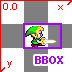
\includegraphics{resources/bbox.png}
  \caption{Link sprite bounding box}
  \label{fig:Link sprite bounding box}
\end{figure}

De plus, pour rajouter une barre de vie pour Zelda et implémenter les fonctions
\emph{pause} et \emph{resume}, nous avons été contraints de dupliquer les
classes GameDefaultImpl et GameLevelDefaultImpl.


\newpage
\section{Architecture du jeu}

\begin{figure}[ht!]
  \center
  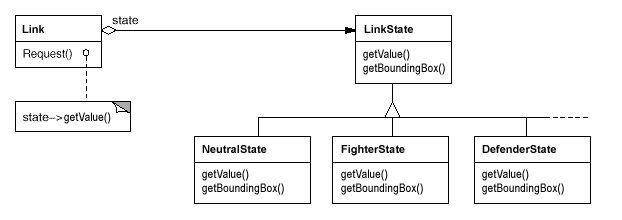
\includegraphics[width=16cm,keepaspectratio]{resources/state_pattern.png}
  \caption{State pattern}
  \label{fig:State pattern}
\end{figure}


\section{Problèmes rencontrés}
La modification des bounding box engendrée par l'utilisation de sprites de
tailles différents a été complexe car il a fallu intégrer les modifications au
système de gestion des collisions.
L'implémentation des fonctions \emph{pause} et \emph{resume} s'est avérée assez
délicate à cause de la gestion des Threads avec les méthodes \emph{wait()} et
\emph{notify()} en étant \emph{synchronized}.
